\documentclass[a4paper, 10pt]{report}
\usepackage[italian]{babel}
\usepackage[T1]{fontenc}
\usepackage[utf8]{inputenc}
\usepackage{charter}
\usepackage{amsmath}
\usepackage{amsthm}
\usepackage{amsfonts}
\usepackage{graphicx}
\usepackage{wrapfig}
\usepackage{tcolorbox}
\usepackage{fancyhdr}
\usepackage{listings}
\usepackage{longtable}
\usepackage{multicol}
\usepackage{xcolor}

\usepackage{geometry}
\geometry{a4paper, left=2cm,right=2cm,top=2cm,bottom=2cm}

\pagestyle{fancy}
\lhead{}
\chead{}
\rhead{\bfseries 17 ottobre 2019 }
\lhead{\bfseries Segnali e immagini - laboratorio}

\newcounter{main}
\setcounter{main}{1}

\lstnewenvironment{code}[1][firstnumber=\themain,name=main]
  {\lstset{language=matlab,
           basicstyle=\medium\ttfamily,
           numbers=left,
           basicstyle=\small,
           columns=fullflexible,
           #1
          }
}
{\setcounter{main}{\value{lstnumber}}}


\begin{document}

\noindent \textbf{Esempio di cross - correlazione per ogni punto di shift:}

\begin{code}
f1 = [1 1 1 1 1 1 1 1]; %box 
f2 = [1 2 3 4 5 6 7 8]; %triangolo

M = length(f1);
N = length(f2);
if N>M 
    f1 = cat(2,f1,zeros(1,N-M));
    M=N;
elseif N<M
    f2 = cat(2,f2,zeros(1,M-N));
end

figure; set(gcf,'name','Cross Correlazione animazione','IntegerHandle','off');
subplot(511); stem(f1); title('f1')
subplot(512); stem(f2); title('f2')

tf1 = [zeros(1,M-1),f1,zeros(1,M-1)];
tf2 = [f2,zeros(1,2*M-2)];

lag = [-M+1:M-1];
MYf1xf2 = [];
for i=1:2*M-1
    subplot(513); stem(tf1); title('f1 allineato')
    subplot(514); stem(tf2); title('f2 allineato')
    MYf1xf2 = [MYf1xf2 sum(tf1.*tf2)];
    tf2 = circshift(tf2,1,2);
    subplot(515); stem(lag(1:i),MYf1xf2); axis([-M+1, M-1,0,40]);
    pause;
end
hold on; subplot(515); plot(lag(1:i),MYf1xf2); 
\end{code}

\noindent \\Analisi codice:

\begin{longtable}{| p{.20\textwidth} | p{.75\textwidth} |}

\textbf{zeros(n, m)} & Crea una matrice nxm di zeri.
\\
\hrule & \hrule
\\
\textbf{circshift(A,K,dim)} & Shifta in modo circolare gli elementi di A di K posizioni. Il valore dim (intero scalare) indica su che dimensione lavorare.

Esempio:

dim = 1 -> gli scambi avvengono per riga (vettori colonna o matrici).

dim = 2 -> gli scambi avvengono per colonna (matrici).
\\
\hrule & \hrule
\\
\textbf{pause} & Mette in pausa l'esecuzione del codice. Per riprendere basta premere "invio".
\\
\end{longtable}

\noindent Osservazioni:
\begin{itemize}
\item[-] Le righe 6-11 eseguono l'operazione di zero padding, ovvero aggiungono zeri ad uno dei due segnali affinchè entrambi abbaino la stesas dimensione. Questo semplifica la cross - correlazione;
\item[-] Le variabili tf1 e tf2 sono "lunghe" 7+8+7, ovvero coprono tutti i punti di shift della cross - correlazione.
\item[-] L'operatore \textbf{.*} esegue l'operazione di moltiplicazione puntuale.

Esempio:
\begin{align*}
\begin{bmatrix} 1&2\\3&4
\end{bmatrix}
\cdot^*
\begin{bmatrix} -2&5\\0&3
\end{bmatrix}
=
\begin{bmatrix} -2&10\\0&12
\end{bmatrix}
\end{align*}

\item[-] Alla riga 25, MYf1xf2 = se stesso concatenato a ...;
\end{itemize}

\newpage

\noindent Risultato:
\begin{center}
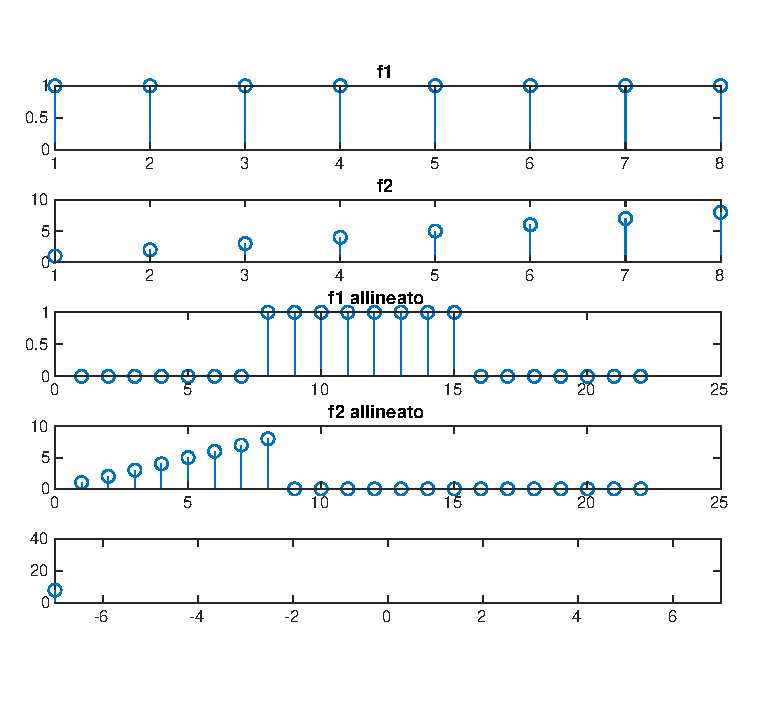
\includegraphics[scale=1]{es2pt1.pdf}

(primo ciclo)

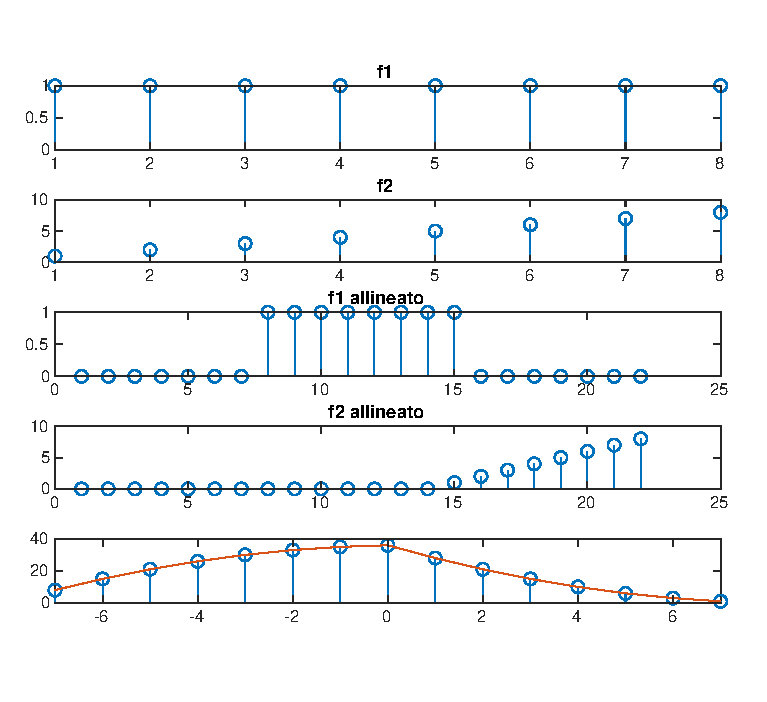
\includegraphics[scale=1]{es2pt3.pdf}

(ciclo finale)
\end{center}


\end{document}